%\documentclass[a4paper]{article}
%% Language and font encodings
\documentclass[twocolumn,aps,prl]{revtex4-1}
\usepackage[utf8]{inputenc}
\usepackage[spanish, es-tabla]{babel}
\usepackage[T1]{fontenc}
\usepackage{amsmath}
\usepackage{amssymb}
\usepackage{siunitx}
\usepackage{multirow}
\usepackage{float}
\usepackage{enumitem} % enumerar

\sisetup{math-micro=\text{µ},text-micro=µ}

\usepackage[toc,page]{appendix}

%% Sets page size and margins
\usepackage[a4paper,top=1.0cm,bottom=1.0cm,left=1.7cm,right=1.7cm,marginparwidth=1.75cm]{geometry}

%% Sets caption text size(its bigger than text)
\usepackage{caption}
\captionsetup[figure]{font=small}
\usepackage{subcaption}

%% Useful packages
\usepackage{svg}
\usepackage{epstopdf}
\usepackage{amsmath}
\usepackage{graphicx}
\usepackage[colorlinks=true, allcolors=blue]{hyperref}

% \newcommand{\nstar}{n^*} 
% \newcommand{\Nstar}{N^*} 

% \newcommand{\N_simulaciones_b}{5000}
\newcommand{\nSimulacionesB}{5000}
\newcommand{\Nsteps}{50}

\newcommand*\sepline{%
  \begin{center}
    \rule[1ex]{.5\textwidth}{.1pt}
  \end{center}}

%%%%%%%%%%%%%%%%%%%%%%%%%%%%%%%%%%%%%%%%%%%%%%%%%%%%%%
%%%%%%%%%%%%%%%%%%%%%%%%%%%%%%%%%%%%%%%%%%%%%%%%%%%%%%

\begin{document}

% ██   ██ ███████  █████  ██████
% ██   ██ ██      ██   ██ ██   ██
% ███████ █████   ███████ ██   ██
% ██   ██ ██      ██   ██ ██   ██
% ██   ██ ███████ ██   ██ ██████

\title{Práctico 3}
\author{M. G. Aramayo}
\affiliation{Matemática de sistemas biológicos, Instituto Balseiro}

% \begin{abstract}
% Mete acá las conclusiones.
% \end{abstract}

\maketitle

\section{Resolución Ej 1}
% ███████╗██╗  ██╗ ██╗
% ██╔════╝╚██╗██╔╝███║
% █████╗   ╚███╔╝ ╚██║
% ██╔══╝   ██╔██╗  ██║
% ███████╗██╔╝ ██╗ ██║
% ╚══════╝╚═╝  ╚═╝ ╚═╝

%**********
\begin{figure*}[ht!]
  \centering
  \begin{subfigure}[b]{0.49\linewidth}
      \centering
      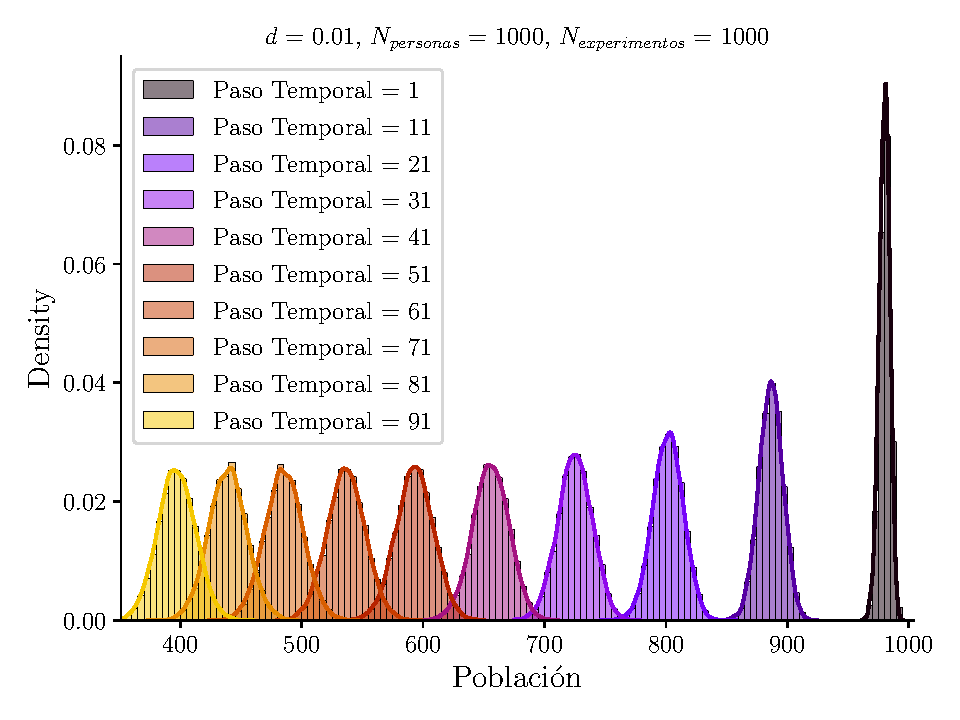
\includegraphics[width = 0.999\textwidth]{figuras/ex01-a-evolucion_temporal.pdf}
      % \caption{Evolución en pasos temporales de la distribución de numero de habitantes.}
      \label{fig:figuras/ex01-a-evolucion_temporal}
  \end{subfigure}
%   \caption{}
  %\label{fig:figuras/ex01-a-evolucion_temporal}
% \end{figure*}
% \begin{figure*}[ht!]
%   \centering
  \begin{subfigure}[b]{0.49\linewidth}
      \centering
      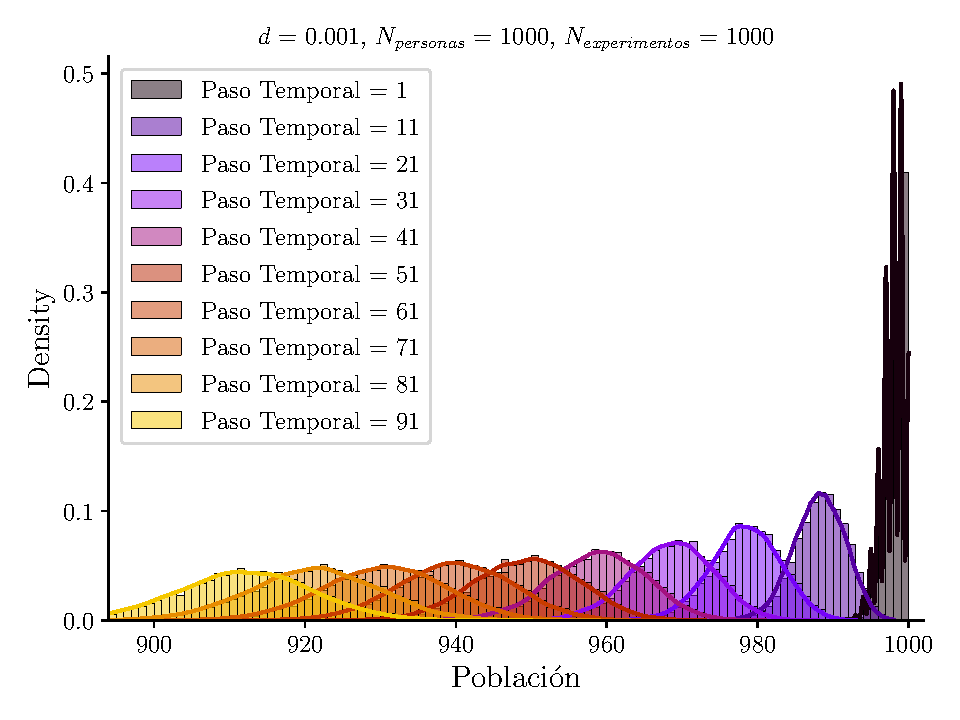
\includegraphics[width = 0.999\textwidth]{figuras/ex01-b-evolucion_temporal.pdf}
      % \caption{Evolución en pasos temporales de la distribución de numero de habitantes.}
      \label{fig:figuras/ex01-b-evolucion_temporal}
  \end{subfigure}
  \caption{Evolución en pasos temporales de la distribución de número de habitantes. Para $d=0.01$ y $d=0.001$. }
  \label{fig:figuras/ex01-evolucion_temporal}
\end{figure*}

\begin{figure*}[ht!]
  \centering
  \begin{subfigure}[b]{0.49\linewidth}
      \centering
      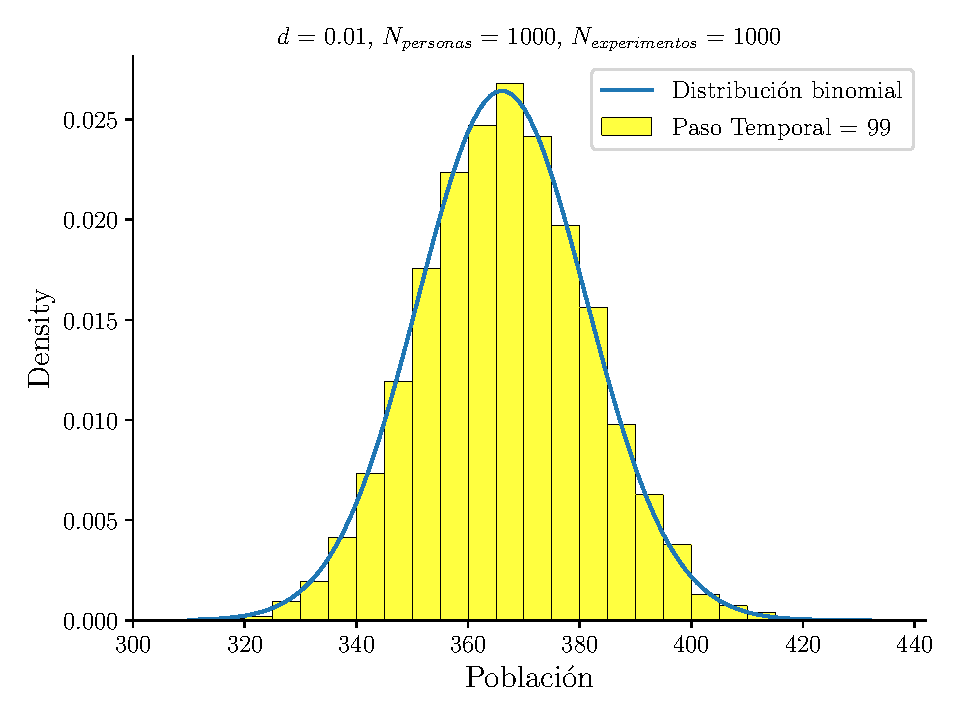
\includegraphics[width = 0.999\textwidth]{figuras/ex01-a-ultima_iteracion.pdf}
      % \caption{Comparación entre la densidad obtenida mediante la   simulación y una distribución binomial.}
      \label{fig:figuras/ex01-a-ultima_iteracion}
  \end{subfigure}
%   \caption{}
%   \label{fig:figuras/ex01-a-ultima_iteracion}
% \end{figure*}
% \begin{figure*}[ht!]
%   \centering
  \begin{subfigure}[b]{0.49\linewidth}
      \centering
      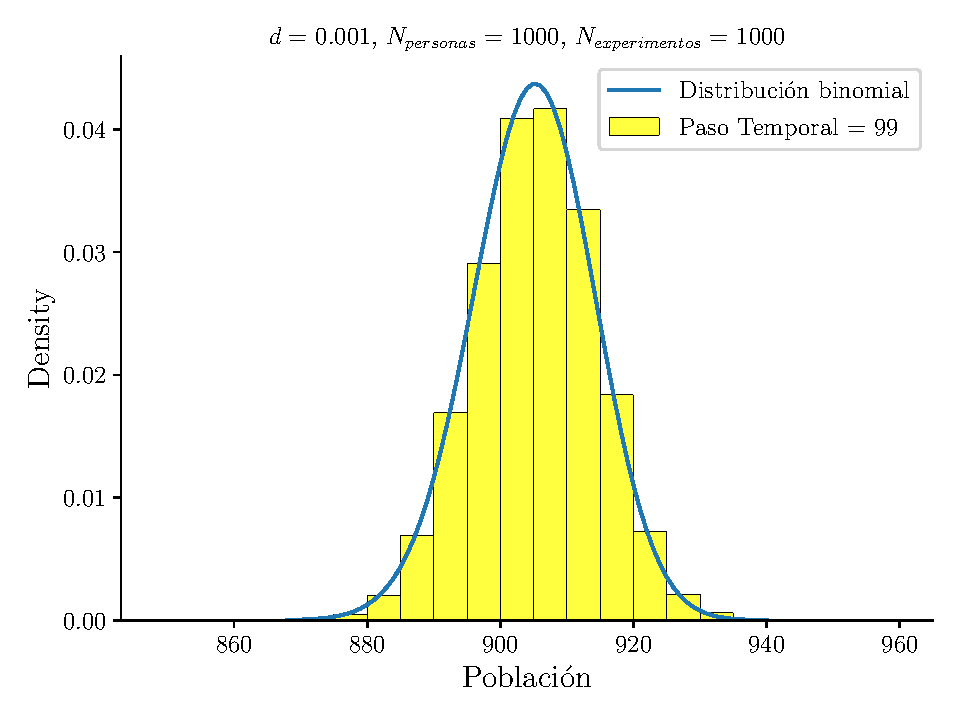
\includegraphics[width = 0.999\textwidth]{figuras/ex01-b-ultima_iteracion.pdf}
      % \caption{Comparación entre la densidad obtenida mediante la   simulación y una distribución binomial.}
      \label{fig:figuras/ex01-b-ultima_iteracion}
  \end{subfigure}
  \caption{Comparación entre la densidad obtenida mediante la simulación y una distribución binomial. Para $d=0.01$ y $d=0.001$.}
  \label{fig:figuras/ex01-ultima_iteracion}
\end{figure*}

Se simula una población de individuos que no se reproducen y evolucionan en tiempo discreto. En cada paso de tiempo cada uno puede morir con probabilidad $d$. Si realizamos varias de estas simulaciones pueden obtenerse las distribuciones de probabilidad en la Fig. \ref{fig:figuras/ex01-evolucion_temporal}. La distribución final parece seguir la forma de una distribución binomial como puede verse en la Fig. \ref{fig:figuras/ex01-ultima_iteracion}.

\section{Resolución Ej 2}
% ███████╗██╗  ██╗    ██████╗  
% ██╔════╝╚██╗██╔╝    ╚════██╗
% █████╗   ╚███╔╝      █████╔╝
% ██╔══╝   ██╔██╗     ██╔═══╝ 
% ███████╗██╔╝ ██╗    ███████╗
% ╚══════╝╚═╝  ╚═╝    ╚══════╝

Se tiene un modelo de población continua de dinámica discreta dado por:
\begin{equation}\label{ec:map01}
  x_{n+1} = a x_n + z_n
\end{equation}
donde $z_n$ es una variable estocástica con distribución gaussiana con media cero y desviación estándar $\sigma$. Esta expresión recursiva no es tan rápida en algunos lenguajes de programación. Pero puede reescribirse, veamos como se comporta a distintos valores de $n$:
\begin{equation}\label{ec:map01-evaluations}
  x_0 = x_0 \Rightarrow
  \left\vert\begin{aligned}
    % x_0 &=     x_0 \\
    x_1 &= a^1 x_0 + a^0 z_0 \\
    x_2 &= a^2 x_0 + a^1 z_0 + a^0 z_1 \\
    % x_3 &= a^3 x_0 + a^2 z_0 + a^1 z_1 + a^0 z_2\\
        & \qquad \qquad \vdots \\
    x_n &= a^n x_0 + a^{n-1} z_0 + \ldots + a^0 z_{n-1}\\
  \end{aligned}\right. , 
\end{equation}
con esto proponemos que puede reescribirse como:
\begin{equation}\label{ec:map01-r}
  x_n = a^{n} x_0 + \sum_{i=0}^{n-1} a^{n-(1+i)} \ z_i
\end{equation}
Una rápida prueba inductiva de que esto es cierto:
$$
\left|
\begin{aligned}
  & \text{Caso base: } x_1 = a^{1} x_0 + \sum_{i=0}^{1-1} a^{1-(1+i)} \ z_i = a^{1} x_0 +z_0\\
  & \text{Asumo validez en $n=k$: } x_k = a^{k} x_0 + \sum_{i=0}^{k-1} a^{k-(1+i)} z_i\\
  & \text{Probar que esto implica validez en $n=k+1$:} \\
  x_{k+1} &= a x_k + z_k = a (a^{k} x_0 + \sum_{i=0}^{k-1} a^{k-(1+i)} z_i) + z_k \\
  x_{k+1} &= a^{k+1} x_0 + a\sum_{i=0}^{k-1} a^{k-(1+i)} z_i + z_k \\
  % x_{k+1} &= a^{k+1} x_0 + \sum_{i=0}^{k-1} \underbrace{a^{k+1-(1+i)} z_i}_{b_{k,i}} + z_k \\
  x_{k+1} &= a^{k+1} x_0 + \sum_{i=0}^{k-1} \underbrace{a^{k+1-(1+i)} z_i}_{b_{k,i}} + \underbrace{a^0 z_k}_{b_{k,k}} \\
  x_{k+1} &= a^{k+1} x_0 + \sum_{i=0}^{k} a^{k+1-(1+i)} z_i \\
  & \text{$\therefore$ se cumple para $n=k+1$}
\end{aligned}
\right.
$$

\begin{figure*}[ht!]
  \centering
  \begin{subfigure}[b]{0.49\linewidth}
      \centering
      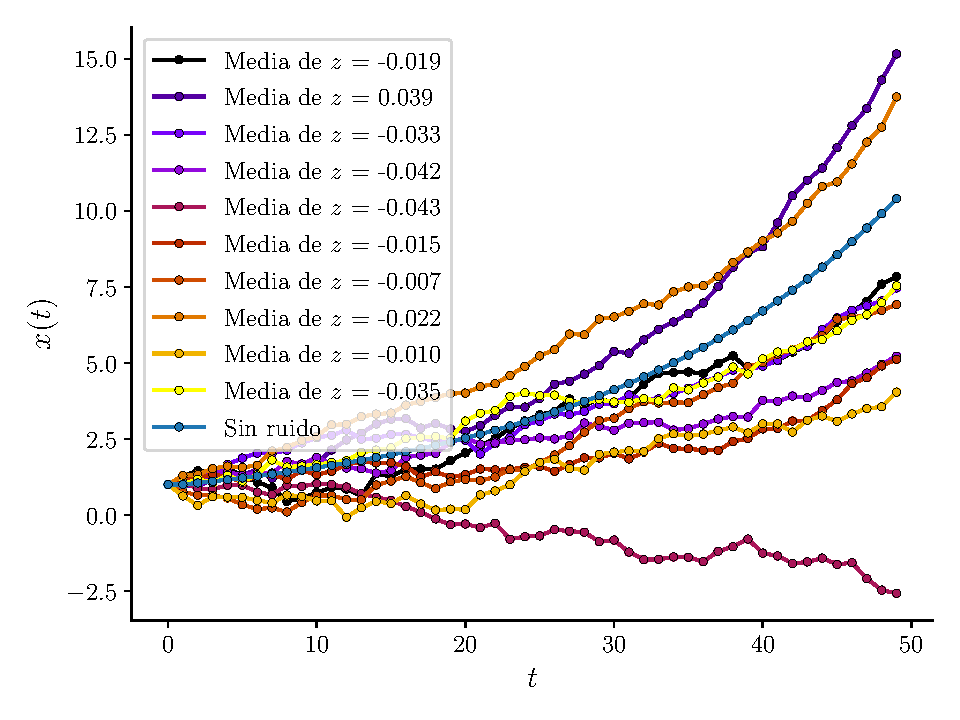
\includegraphics[width = 0.999\textwidth]{figuras/ex02-mapeo.pdf}
      \caption{Evolución del mapeo para distintos valores medios de la generación de números aleatorios, para $\Nsteps$ pasos en $t$.}
      \label{fig:figuras/ex02-mapeo}
  \end{subfigure}
  % \caption{}
  %\label{fig:figuras/ex02-mapeo}
% \end{figure*}
% \begin{figure*}[ht!]
%   \centering
  \begin{subfigure}[b]{0.49\linewidth}
      \centering
      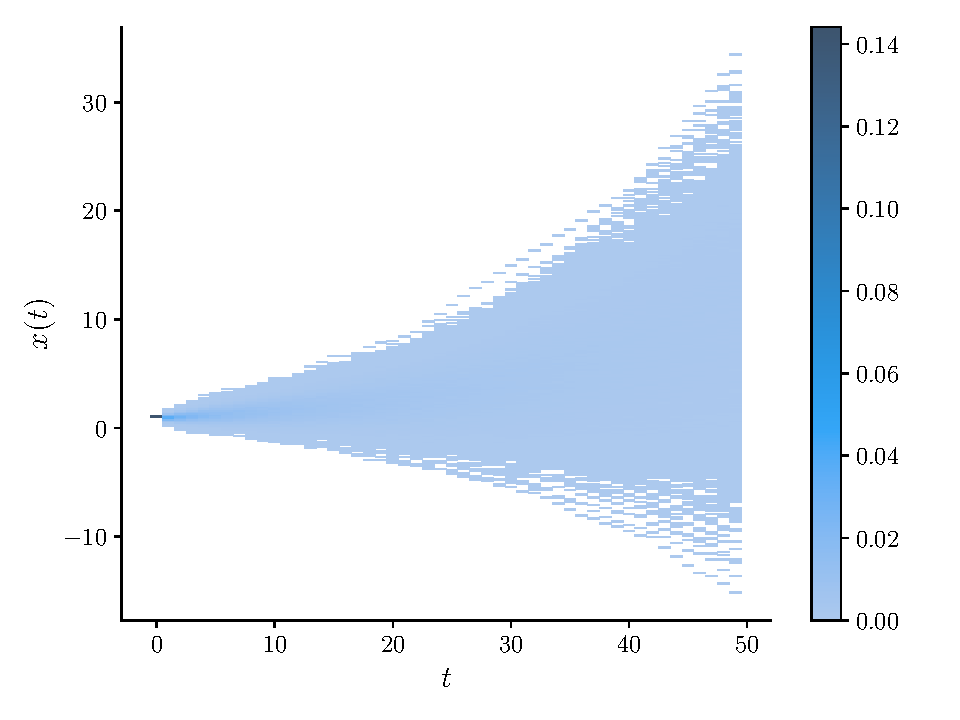
\includegraphics[width = 0.999\textwidth]{figuras/ex02-histograma.pdf}
      \caption{$P(x,t)$ densidad de probabilidad (color) de $x$ y $t$ calculada a partir de $\nSimulacionesB$ evaluaciones de $\Nsteps$ pasos en $t$.}
      \label{fig:figuras/ex02-histograma}
  \end{subfigure}
  \caption{Mapeo de la Ec. \ref{ec:map01-r}}
  \label{fig:figuras/ex02-0}
\end{figure*}

La expresión de la Ec. \ref{ec:map01-r} se utilizó para realizar múltiples simulaciones en la Fig. \ref{fig:figuras/ex02-mapeo}. Para un número mayor de simulaciones puede obtenerse la distribución $P(x,t)$ del sistema, el resultado se puede ver en la Fig. \ref{fig:figuras/ex02-histograma}.
%%%%%%%%%%%%%%%%%%%%%%%%%%%%%%%%%%%%%%%%%%%%%%%%%%%%%%%%%%%%%%%%
\sepline
%%%%%%%%%%%%%%%%%%%%%%%%%%%%%%%%%%%%%%%%%%%%%%%%%%%%%%%%%%%%%%%%
Por otro lado, un segundo modelo de población continua de dinámica discreta dado por:
\begin{equation}\label{ec:map02}
  x_{n+1} = (a + z_n) x_n
\end{equation}
donde $z_n$ es una variable estocástica con distribución gaussiana con media cero y desviación estándar $\sigma$. Nuevamente, puede reescribirse de forma no recursiva.

Veamos como se comporta a distintos valores de $n$:
\begin{equation}
  x_0 = x_0 \Rightarrow
  \left\vert\begin{aligned}
    % x_0 &=     x_0 \\
    x_1 &= x_0 (a + z_0) \\
    x_2 &= x_0 (a + z_0) (a + z_1)\\
        & \qquad \qquad \vdots \\
    x_n &= x_0 (a + z_0) (a + z_1) ... (a + z_{n-1})\\
  \end{aligned}\right.
\end{equation}

Puede reescribirse como:
\begin{equation}\label{ec:map02-r}
  x_n = x_0 \prod_{i=0}^{n-1} (a + z_i)
\end{equation}
Una rápida prueba inductiva de que esto es cierto:

\begin{equation}
  \left|
  \begin{aligned}
    & \text{Un ejemplo de que se cumple:} \\
    x_1 &= x_0 \prod_{i=0}^{1-1} (a + z_i) = x_0 (a + z_0)\\
    & \text{Asumo que se cumple para $n=k$:} \\
    x_k &= x_0 \prod_{i=0}^{k-1} (a + z_i)\\
    & \text{Probar que esto implica que se cumple para $n=k+1$:} \\
    x_{k+1} &= (a + z_k) x_k = (a + z_k) x_0 \prod_{i=0}^{k-1} (a + z_i) \\
    x_{k+1} &= (a + z_k) x_0 \prod_{i=0}^{k-1} (a + z_i) \\
    x_{k+1} &= x_0 \prod_{i=0}^{k} (a + z_i) \\
    & \text{$\therefore$ se cumple para $n=k+1$}
  \end{aligned}
  \right.  
\end{equation}

\begin{figure*}[ht!]
  \centering
  \begin{subfigure}[b]{0.49\linewidth}
    \centering
    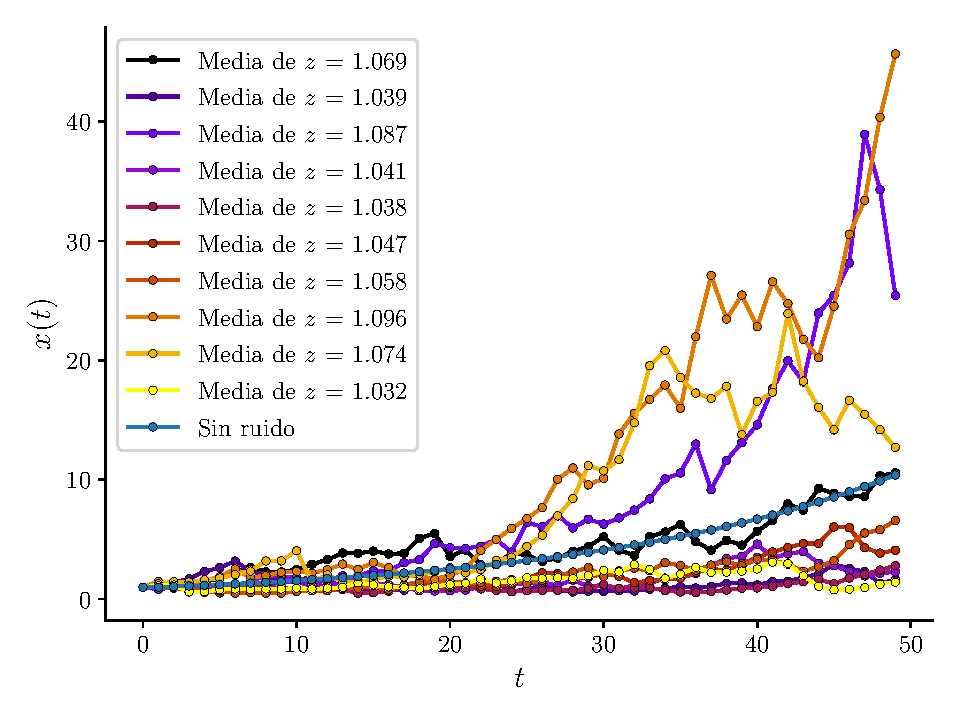
\includegraphics[width = 0.999\textwidth]{figuras/ex02-mapeo-02.pdf}
    \caption{Evolución del mapeo para distintos valores medios de la generación de números aleatorios, para $\Nsteps$ pasos en $t$.}
    \label{fig:figuras/ex02-mapeo-02}
  \end{subfigure}
  % \caption{}
  %\label{fig:figuras/ex02-mapeo-02}
  % \end{figure*}
  % \begin{figure*}[ht!]
    %   \centering
  \begin{subfigure}[b]{0.49\linewidth}
    \centering
    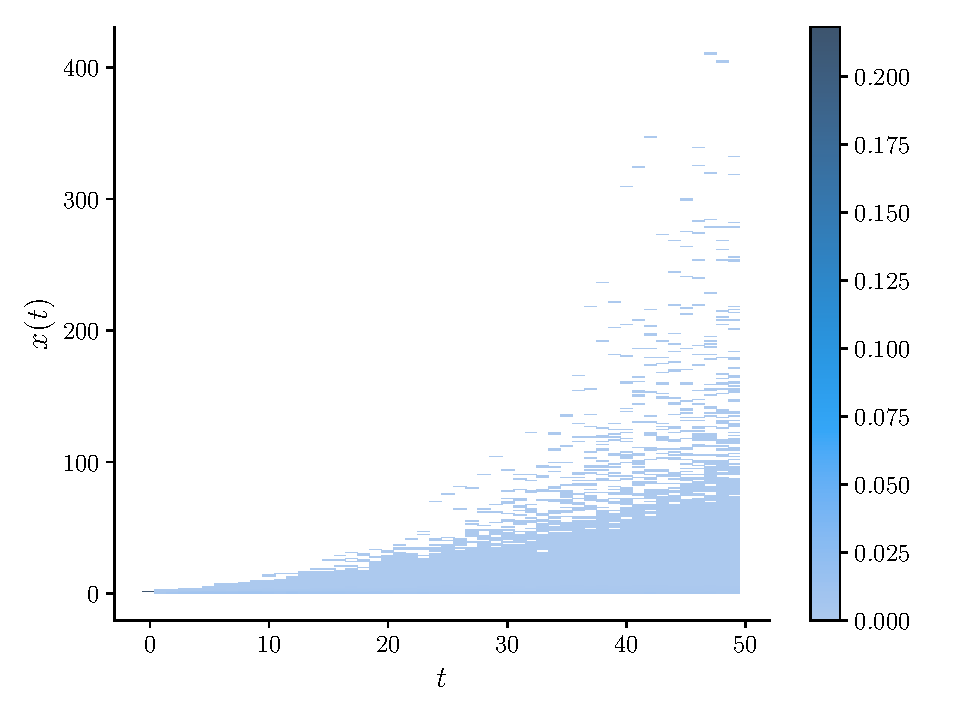
\includegraphics[width = 0.999\textwidth]{figuras/ex02-histograma-02.pdf}
    \caption{$P(x,t)$ densidad de probabilidad (color) de $x$ y $t$ calculada a partir de $\nSimulacionesB$ evaluaciones de $\Nsteps$ pasos en $t$.}
    \label{fig:figuras/ex02-histograma-02}
  \end{subfigure}  
  \caption{Mapeo de la Ec. \ref{ec:map02-r}.}
  \label{fig:figuras/ex02-02}
\end{figure*}

La expresión de la Ec. \ref{ec:map02-r} se utilizó para realizar múltiples simulaciones en la Fig. \ref{fig:figuras/ex02-mapeo-02}. Para un número mayor de simulaciones puede obtenerse la distribución $P(x,t)$ del sistema, el resultado se puede ver en la Fig. \ref{fig:figuras/ex02-histograma-02}.

\section{Resolución Ej 3}

% ███████╗██╗  ██╗    ██████╗     
% ██╔════╝╚██╗██╔╝    ╚════██╗    
% █████╗   ╚███╔╝      █████╔╝    
% ██╔══╝   ██╔██╗      ╚═══██╗    
% ███████╗██╔╝ ██╗    ██████╔╝    
% ╚══════╝╚═╝  ╚═╝    ╚═════╝     

\begin{figure*}[ht!]
  \centering
  \begin{subfigure}[b]{0.49\linewidth}
      \centering
      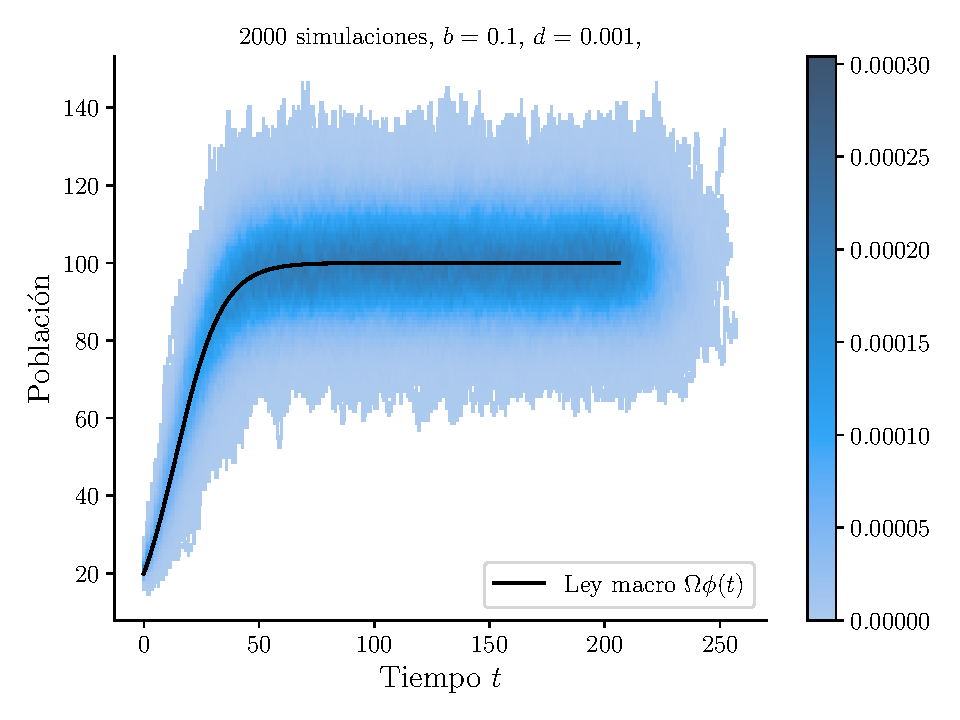
\includegraphics[width = 0.999\textwidth]{figuras/ex03-a-SinCota.pdf}
      \caption{Distribución $P(N_A,t)$ (en color) calculada numéricamente.}
      \label{fig:figuras/ex03-a-SinCota}
  \end{subfigure}\quad
%   \caption{}
%   \label{fig:figuras/ex03-a-SinCota}
% \end{figure*}
% \begin{figure*}[ht!]
%   \centering
  \begin{subfigure}[b]{0.49\linewidth}
      \centering
      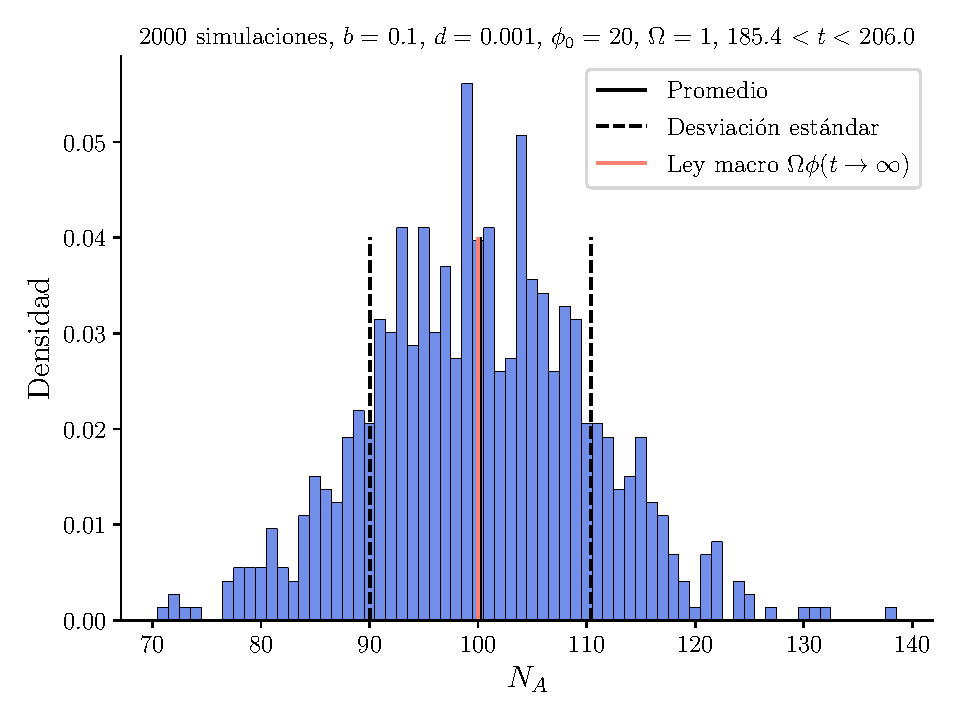
\includegraphics[width = 0.999\textwidth]{figuras/ex03-b-SinCota.pdf}
      \caption{Distribución de poblaciones en el estado estacionario. Las barras indican las predicciones teóricas y predichas mediante múltiples simulaciones.}
      \label{fig:figuras/ex03-b-SinCota}
  \end{subfigure}\quad
  \caption{Simulación de Ec. \ref{ec:gillespie} con población media estacionaria no nula.}
  \label{fig:figuras/ex03-stat}
\end{figure*}

Se utilizó el algoritmo de Gillespie para simular una población mediante un modelo de reproducción y competencia intraespecífica con tasas $b$ y $d$ de los procesos:
\begin{equation}\label{ec:gillespie}
  \begin{aligned}
    A & \stackrel{b}{\rightarrow} A+A \\
    A+A & \stackrel{d}{\rightarrow} A
  \end{aligned}
\end{equation}

Es posible obtener una ecuación diferencial que modele este sistema a partir de las tasas de transición son:
\begin{equation}
  \begin{aligned}
    T(A-1 \mid A) &= d \frac{A}{N} \frac{A}{N} 
    = d\frac{A^2}{N^2} \\
    T(A+1 \mid A) &= b \frac{A}{N}
  \end{aligned}
\end{equation}

Si se tiene $A=\phi N$ con $0<\phi<1$:
\begin{equation}
  \begin{aligned}
    T(A-1 \mid A) &= d \phi^{2} \\
    T(A+1 \mid A) &= b \phi
  \end{aligned}
\end{equation}
Con esto en cuenta la propuesta de ecuación es:
  $\dot{\phi}=b \phi-d \phi^{2}$
con lo que $r=b, s=d$ son parámetro de la función logística:
\begin{equation}
  \phi(t)=\frac{r}{s-c e^{-r t}}, c=s-\frac{r}{\phi_{0}}
\end{equation}

Esta ecuación, escalada al tamaño macroscópico, permite modelar el tamaño de $A$ luego de sus transiciones.

Con esto en cuenta, se encontraron parámetros que permiten un valor medio de población estacionario no nulo que puede verse en la Fig. \ref{fig:figuras/ex03-stat}. Se grafica junto con su modelo macroscópico.

\begin{figure*}[ht!]
  \centering
  \begin{subfigure}[b]{0.49\linewidth}
      \centering
      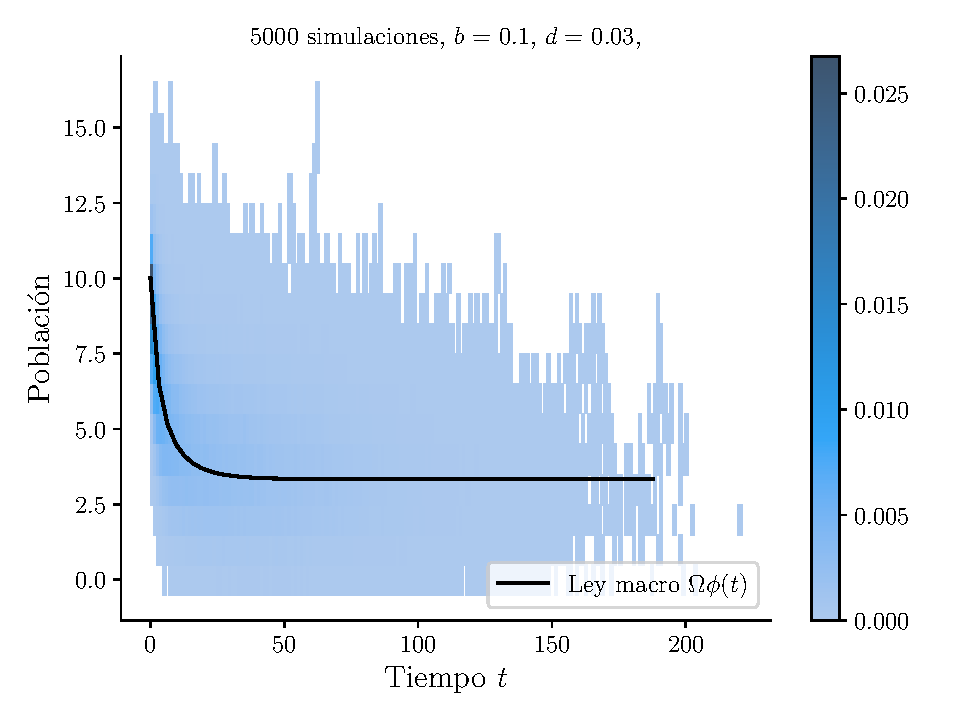
\includegraphics[width = 0.999\textwidth]{figuras/ex03-c-SinCota.pdf}
      \caption{Distribución $P(N_A,t)$ (en color) calculada numéricamente.}
      \label{fig:figuras/ex03-c-SinCota}
  \end{subfigure}\quad
%   \caption{}
%   \label{fig:figuras/ex03-c}
% \end{figure*}
% \begin{figure*}[ht!]
%   \centering
  \begin{subfigure}[b]{0.49\linewidth}
      \centering
      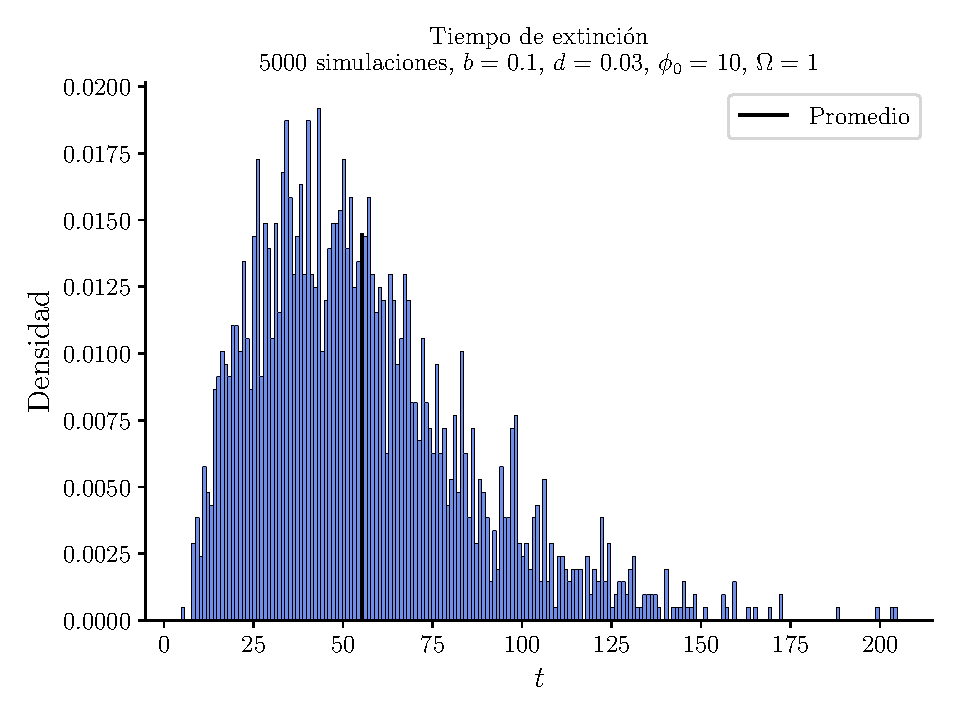
\includegraphics[width = 0.999\textwidth]{figuras/ex03-e-SinCota.pdf}
      \caption{Distribución de tiempos de extinción.}
      \label{fig:figuras/ex03-e-SinCota}
  \end{subfigure}\quad
  \caption{Simulación de Ec. \ref{ec:gillespie} con extinción.}
  \label{fig:figuras/ex03-kill}
\end{figure*}
%**********

Se obtuvo un conjunto de parámetros que producen una extinción, resultados asociados a esta simulación pueden verse en la Fig. \ref{fig:figuras/ex03-kill}.

% \begin{figure*}[ht!]
%   \centering
%   \begin{subfigure}[b]{0.33\linewidth}
%       \centering
%       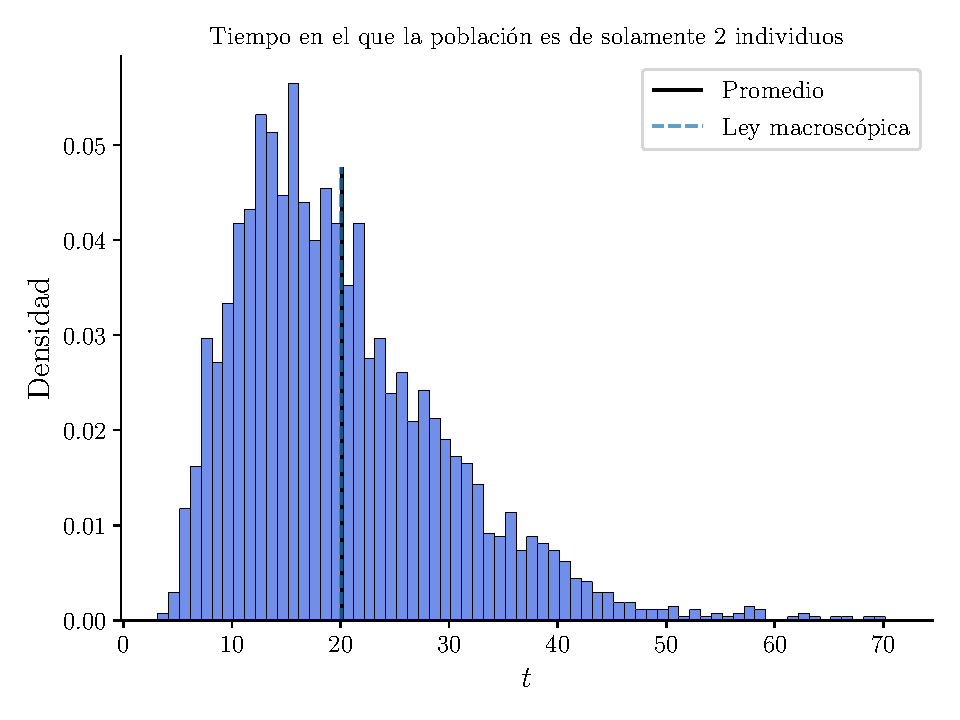
\includegraphics[width = 0.9\textwidth]{figuras/ex03-d.pdf}
%       \caption{}
%       \label{fig:figuras/ex03-d}
%   \end{subfigure}\quad
%   \caption{}
%   %\label{fig:figuras/ex03-d}
% \end{figure*}

\end{document}